% =====================================================================
%  Anticipation, Not Reaction
%  Media Discourse, FOMC Communication, and Pre-Announcement Volatility
%  Wang and Jin (2026). Compile with pdfLaTeX (bibtex).
% =====================================================================
\documentclass[11pt,a4paper]{article}

\usepackage[utf8]{inputenc}
\usepackage[T1]{fontenc}
\usepackage[margin=2.4cm]{geometry}
\usepackage{setspace}
\onehalfspacing

\usepackage{booktabs}
\usepackage{tabularx}
\usepackage{array}
\usepackage{amsmath,amssymb}
\usepackage{graphicx}
\usepackage{titlesec}
\usepackage{fancyhdr}
\usepackage{caption}
\usepackage{enumitem}
\usepackage{hyperref}
\usepackage{xurl}
\usepackage{natbib}

\graphicspath{{figures/}}
\hypersetup{hidelinks, pdftitle={Anticipation, Not Reaction}}
\urlstyle{same}
\captionsetup{font=small,labelfont=bf}
\emergencystretch=3em
\sloppy

\newcommand{\simk}[1]{\ensuremath{\mathrm{sim}_{#1}}}

\titleformat{\section}{\large\bfseries}{\thesection}{0.5em}{}
\titleformat{\subsection}{\normalsize\bfseries}{\thesubsection}{0.5em}{}

\pagestyle{fancy}\fancyhf{}
\rhead{\small Wang and Jin (2026)}
\lhead{\small Anticipation, Not Reaction}
\rfoot{\small \thepage}
\setlength{\headheight}{14pt}

\title{\textbf{Anticipation, Not Reaction:}\\[3pt]
\large Media Discourse, FOMC Communication, and Pre-Announcement Volatility,
2015--2025}

\author{
Duo (Doris) Wang\thanks{Corresponding author. The University of Chicago. Email:
\texttt{dorisduowang@uchicago.edu}.}
\quad\quad
Yuzhao (Jerry) Jin\thanks{The University of Chicago. Email:
\texttt{yuzhaojin1@uchicago.edu}.}
}
\date{This draft: \today}

\begin{document}
\maketitle
\thispagestyle{fancy}

% =====================================================================
\begin{abstract}
\noindent
Federal Reserve communication has become a policy instrument in its own right,
and a large literature reads the language of the Federal Open Market Committee
(FOMC) as a signal that travels through the news media to markets. Most of that
work rests on a single outlet and a few hundred articles. We ask, at the scale of
United States Federal Reserve news coverage, whether media discourse around FOMC
meetings anticipates, mirrors, or follows the official minutes, and whether
pre-meeting textual alignment between the media and the minutes helps predict
realized stock-market volatility. We build a distributed pipeline that scores tone
across roughly 2.36 million Global Database of Events, Language and Tone (GDELT)
records together with Federal Reserve coverage from The New York Times and The
Guardian, and we measure media--FOMC similarity in the days around each of the
88 meetings from 2015 to 2025. Two days before a meeting, broad media coverage is
most strongly associated with post-meeting volatility: the raw correlation is
$0.56$ ($p<0.001$) and survives a permutation placebo, a leave-one-out check, and
a bootstrap whose confidence interval excludes zero. The signal does not, however,
represent an independent media channel. Once we condition on the prevailing level
of the VIX and on pre-meeting volatility, the coefficient falls by roughly
four-fifths and is no longer distinguishable from its permutation null. We read
the pattern as joint processing of a common latent macro-uncertainty state rather
than as media causing markets, a reading the identification battery supports and
that an independent measurement result reinforces: scored with the Loughran--McDonald
market dictionary, the negative tone of the minutes moves with the pre-meeting VIX
($r=0.52$) and forecasts post-meeting realized volatility, so the Committee's own
language is most negative exactly where priced uncertainty is highest. The
contribution is empirical and methodological in that order: a staged identification
design that separates pre-meeting information alignment from post-announcement
reaction and shows where a causal reading fails; a tone measure anchored to the
market rather than to a second word list; and, enabling both, a reproducible
pipeline that assembles and scores monetary-policy text at population scale.\\[6pt]
\noindent\textbf{Keywords:} central bank communication; FOMC; textual similarity;
realized volatility; rational inattention; GDELT.\\
\noindent\textbf{JEL:} E52, E58, G14, G41.
\end{abstract}

\noindent\textbf{Highlights}
\begin{itemize}[leftmargin=1.3em,itemsep=1pt,topsep=2pt]
  \item Pre-meeting media--FOMC similarity correlates with post-meeting volatility at $r=0.56$.
  \item The signal peaks two days before the meeting, not after it.
  \item Controlling for the VIX and prior volatility shrinks the effect by four-fifths.
  \item Placebo, surprise, Granger, and bootstrap tests point to joint macro processing.
  \item Market-dictionary tone of the minutes moves with the VIX ($r=0.52$), anchoring the measure.
\end{itemize}

% =====================================================================
\section{Introduction}
\label{sec:intro}

For two decades the words of the Federal Reserve have carried at least as much
market-moving weight as its rate decisions. Policy moves are sparse, a handful of
changes in a typical year, but the Committee communicates almost continuously
through statements, minutes, speeches, and testimony. In that environment the
question of how the Fed talks now conveys more information about the near future
than what it has just done, and a broad literature in economics and finance has
come to treat central-bank language as a measurable signal
\citep{blinder2008central,hansen2016shocking}. The signal does not reach investors
directly. It is filtered, summarized, and amplified by the news media, which sits
between the institution and the households and asset managers who form
expectations \citep{tetlock2007giving}.

Most empirical work on this transmission is bounded by its sample. A study reads
one outlet, a few hundred articles, and a hand-built dictionary, and it estimates
a contemporaneous relationship between media tone and prices. That design cannot
separate two very different stories. In the first, the media leads: coverage
carries information about the coming meeting that markets then price. In the
second, media and markets move together because both are reading the same
underlying macroeconomic environment, so any apparent lead is joint determination
through a latent state rather than a causal channel. Distinguishing the two
requires coverage at something closer to the full population of Federal Reserve
news, and it requires a research design built to test for pre-meeting information
rather than to describe post-announcement reaction.

We take up both requirements. We assemble United States Federal Reserve news
coverage at scale, roughly 2.36 million records from the GDELT Global Knowledge
Graph together with phrase-matched coverage from The New York Times and The
Guardian, and we align it in time to the 88 FOMC meetings held between 2015 and
2025. For each meeting we measure the textual similarity between the media
coverage in a given lag day and the eventual FOMC minute, and we relate
pre-meeting similarity to the realized volatility of the S\&P 500 in the days
after the announcement. The central object is \simk{-2}, media--FOMC similarity two
days before the meeting, a lag we fix in advance rather than search for.

Three findings follow. First, the pre-meeting association is real and it is
located before the meeting: the correlation between \simk{-2} and post-meeting
volatility in the broad-coverage GDELT corpus is $0.56$ ($p<0.001$), it is the
strongest point in the lead--lag profile, and it survives a permutation placebo, a
leave-one-out check, and a pairs bootstrap whose ninety-five percent interval
excludes zero. Second, the association is not an independent media channel. Once we
condition on the level of the VIX on the eve of the meeting and on realized
volatility in the prior window, the coefficient on \simk{-2} falls by about
four-fifths and is no longer separable from its permutation null, and the partial
correlation given those controls is $0.14$ with a permutation $p$-value of $0.42$.
Crucially, the coefficient does not recover when we add the high-frequency monetary
policy surprise of \citet{bauer2023reassessment}, so the pre-meeting signal is not
information about the announcement that markets had left unpriced.
Third, the pattern is concentrated in the broad corpus. The two curated outlets,
despite higher same-day topical similarity, show no significant pre-meeting
lead--lag relationship, which is what we expect if breadth and volume, not
editorial selection, drive the population-scale signal.

We read these results as anticipation in the specific sense of joint processing.
Before a meeting, when macroeconomic uncertainty is elevated, the national news
stream writes more language that resembles the Fed's own, and markets
simultaneously widen the distribution of outcomes they price, which shows up as
higher realized volatility once the meeting passes. The media does not move the
Fed and it does not, on this evidence, carry information beyond the common
uncertainty state. That reading is disciplined rather than assumed: it is the
interpretation left standing after the controls, placebo, and dynamic tests, and
it is consistent with a rational-inattention account in which attention flows to
high-variance signals \citep{sims2003implications,mackowiak2009optimal}.

The paper makes three contributions, empirical and methodological in that order.
The first is to identification. We offer a staged design that moves from the raw
correlation to a sequence of controls, then to a high-frequency policy-surprise
test and to placebo, Granger, and bootstrap inference, so that the reader can see
exactly where a causal reading would be warranted and where it collapses; the
central empirical fact, that a large unconditional pre-meeting signal is almost
entirely common macro variation, is established by watching it weaken as each
control enters rather than asserted. The second is to measurement. We score the
Committee's language with an externally fixed market dictionary rather than a
bespoke word list and validate it against the market itself---the VIX, realized
volatility, and the high-frequency surprise---so the tone variable has standing
independent of the authors' judgment. The third, which enables the first two, is a
reproducible pipeline that ingests, scores, and compares monetary-policy text at
population scale; we regard it as infrastructure for the empirical result rather
than as the result. Section~\ref{sec:lit} places the paper in the
literature. Section~\ref{sec:data} describes the corpora and the market data.
Section~\ref{sec:methods} sets out the pipeline and the econometrics.
Section~\ref{sec:results} reports the results. Sections~\ref{sec:discussion}
and~\ref{sec:conclusion} discuss and conclude.

% =====================================================================
\section{Related Literature}
\label{sec:lit}

Because the empirical choices in this paper---what text to read, how to turn it
into a number, what market outcome to explain, and how to control the estimate---
are all borrowed from established practice rather than invented here, we organize
the review around those choices and the literatures that validate each one. The
purpose is less to catalogue what is known than to show that every link in the
measurement chain rests on a method that has already been tested elsewhere.

\subsection{Reading central-bank language, and why the media is the natural next text}

The modern view treats communication as a lever of monetary policy rather than as
commentary on it, and \citet{blinder2008central} draw the distinction that runs
through everything that follows: communication can work through a predictability
effect, telling markets what the Committee will do, or through an information
effect, changing what markets believe about the economy itself. The text-based
generation of this work reads the Committee's own words directly, and it
establishes that doing so is informative. \citet{hansen2016shocking} decompose FOMC
statements with topic models and recover economic-conditions and policy-stance
components with distinct macroeconomic effects; \citet{cieslak2019non} separate
monetary from non-monetary news in central-bank communication; and
\citet{gorodnichenko2023voice} show that even the tone of the Chair's voice carries
information beyond the transcript. The common feature of this strand is that the
text under study is the Fed's own, and its lesson for us is that monetary-policy
language is measurable and priced. The step we take is to read the text that sits
between the institution and the investor rather than the institution's text alone,
because the quantity that households and asset managers actually encounter is the
Fed as filtered through the news. Measuring the alignment between the two texts,
rather than the level of either, is the natural way to ask whether the filter
carries pre-meeting information, and it is the same logic that
\citet{picault2017words} use when they build a field-specific hawkish--dovish
lexicon for European Central Bank communication and relate it to market reactions.

\subsection{Turning text into a number: dictionaries and document similarity}

The measurement side of the paper inherits two now-standard techniques, and it is
worth being explicit about where each comes from because the credibility of the
tone and similarity variables depends on it. The first is the finance dictionary.
General-purpose word lists mislabel financial language, as \citet{loughran2011liability}
showed when they documented that words coded negative in common lexicons are
routinely neutral in financial filings, and the finance-specific dictionary they
built in response---together with the broader program surveyed in
\citet{loughran2020textual}---has become the reference instrument for lexical tone
in finance. Our tone measure is constructed from that dictionary rather than from a
hand-assembled word list precisely so that the mapping from words to sentiment is
fixed externally and is not a researcher degree of freedom, a concern that
\citet{gentzkow2019text} place at the centre of their survey of text as economic
data. The second inherited technique is document similarity. Representing a
document as a term-frequency vector and comparing documents by the cosine of the
angle between those vectors is the workhorse of text-based finance:
\citet{hoberg2016text} use exactly this construction on firm product descriptions
to build time-varying industry classifications, and \citet{cohen2020lazy} use it on
successive corporate filings to show that textual change predicts returns. We apply
the same cosine-similarity construction to a different pair of documents, the news
and the minute, which lets us carry over a validated measurement choice rather than
defend a new one. At the aggregate end, \citet{bybee2024business} treat the entire
news stream as a panel and tie topic-level news flow to the business cycle, and
\citet{shapiro2022measuring} show that a market-validated news-sentiment series can
be built at scale from the full flow of economic reporting; our contribution to
this line is to narrow the frequency from the business cycle to the event window,
so that the news flow can be tied to a discrete policy event and to the market
response in the same window.

\subsection{Media, attention, and the reading of a common state}

That the news can move prices, at least transiently, is the contribution of
\citet{tetlock2007giving}, who show that pessimism in a single financial column
predicts short-horizon downward pressure that later mean-reverts, evidence that
coverage can transmit sentiment rather than only fundamentals. We examine a
pre-event version of that idea at population scale, and the mechanism we have in
mind is not persuasion but shared attention. When attention is costly, agents
direct it toward high-variance signals \citep{sims2003implications,mackowiak2009optimal},
so in the days before an FOMC meeting, as macroeconomic variance rises, journalists
and investors reallocate attention toward Fed-relevant information at the same time
and for the same reason. This is why we are prepared to read a pre-meeting rise in
media--FOMC similarity as joint determination through a common latent state rather
than as the media leading the Fed, and it is why the empirical design below is
built to look for that common state rather than to assume a causal channel. Absent
an instrument that shifts coverage without shifting the economy, the dynamic tests
we report describe lead--lag structure; they are not offered as proof of direction.

\subsection{The market outcome and the controls that discipline it}

The final two choices---the outcome variable and the controls---come from the
asset-pricing side of the literature, and they are what make the exercise a
macro-finance paper rather than a text-mining one. We take realized volatility as
the outcome because volatility, not the signed return, is the quantity a resolution
of uncertainty should move, and because realized volatility computed from daily
returns is a well-understood and consistent estimator of the latent variance
process \citep{andersen2003modeling}. We control for the VIX because implied
volatility is the market's own forward-looking gauge of the uncertainty state, and
because uncertainty measured this way has first-order real and financial
consequences \citep{bloom2009impact}; conditioning on it is therefore the direct
test of whether a media signal is anything more than that common state. Finally, we
control for the high-frequency monetary policy surprise, the component of the
announcement that markets did not anticipate, identified from asset-price movements
in a tight window around the decision in the tradition of \citet{kuttner2001monetary},
\citet{gurkaynak2005sensitivity}, and \citet{nakamura2018high}, and reassessed by
\citet{bauer2023reassessment} to separate pure policy shocks from Fed-information
shocks. The surprise control carries the identification: a pre-meeting media signal
that merely encoded the coming announcement would be absorbed once the surprise is
included, so the fact that our pre-meeting coefficient is already small before the
surprise enters, and does not move when it does, is the evidence that the signal is
not unpriced information about the decision.

\subsection{The gap}

Taken together, the literature establishes that Fed communication is priced, that
dictionary and similarity methods are validated instruments, that the media is an
active intermediary, and that realized volatility conditioned on the VIX and the
policy surprise is the right asset-pricing laboratory for a discrete monetary
event. What is missing is a study that assembles these pieces at the full
population of Federal Reserve news rather than a curated subset, that measures tone
with an externally fixed market dictionary rather than a bespoke list, and that
stages its identification so a reader can see precisely where a causal reading
fails. This paper occupies that intersection.

% =====================================================================
\section{Data}
\label{sec:data}

\subsection{FOMC minutes}

We scrape the minutes of all 88 regularly scheduled FOMC meetings from January
2015 through December 2025 from the Federal Reserve website. Each minute is
cleaned, lower-cased, and tokenized, and it anchors the meeting window used
throughout. The minutes are the reference text against which all media coverage is
compared, and they are also the text on which the market-dictionary tone measure is
computed.

\subsection{GDELT Global Knowledge Graph}

The broad-coverage corpus is the GDELT 2.0 Global Knowledge Graph, a
near-real-time index of world news that we filter to United States sources with
Federal-Reserve-relevant themes and entities. After filtering and windowing to a
band of days around each meeting, the scored corpus contains roughly 2.36 million
records. GDELT is not a curated sample; it is close to the population of United
States news that mentions the Fed, which is exactly what the research question
requires and what a single-outlet study cannot provide \citep{leetaru2013gdelt}.
That breadth comes at a cost in temporal coverage, however, because the
meeting-window similarity panel with complete pre-meeting coverage at a common lag
spans 33 meetings from March 2015 to March 2019. Rather than silently pool meetings
with incomplete windows, we therefore treat those 33 meetings as the estimation
sample for the broad corpus and document the coverage of every corpus explicitly in
Table~\ref{tab:coverage}.

\subsection{Curated outlets}

We complement the broad corpus with phrase-matched ``Federal Reserve'' coverage
from The New York Times and The Guardian, obtained through their article APIs and
extended back to 2015. These outlets are editorially selected and far smaller,
around 61 and 84 covered meetings respectively, and they serve as the contrast
that isolates the role of breadth. If curated selection added signal, these
outlets should lead at least as strongly as GDELT; the results show they do not.

\subsection{Market data}

The outcome is the realized volatility of the S\&P 500 around each meeting,
computed from daily returns as the annualized standard deviation over the trading
days immediately before and after the meeting date. Because a single window is a
choice rather than a fact, we recompute the outcome at windows of three, five,
seven, and ten trading days and report the full set as robustness. We also use the
CBOE Volatility Index (VIX), taken from the Federal Reserve Economic Data service
for the full 2014--2025 span, and we define the pre-meeting VIX as the last close
strictly before the meeting. The VIX matters because it enters as the control that
captures the prevailing level of implied uncertainty on the eve of the meeting,
which is precisely the common state our interpretation turns on.

\subsection{Monetary policy surprises}

To separate a pre-meeting information channel from the announcement itself, we use
the high-frequency monetary policy surprises of \citet{bauer2023reassessment},
distributed by the Federal Reserve Bank of San Francisco. For each meeting the
series records the surprise change in the expected path of the federal funds rate
over the coming year, measured in a tight window around the announcement, together
with an orthogonalized version purged of predictable variation. Every meeting in
the broad-corpus estimation sample matches a surprise observation, so the control
enters without further loss of sample. The logic is direct: if pre-meeting media
similarity merely proxied for the announcement surprise, then including the
surprise should absorb it; that it does not, because the similarity coefficient is
already small before the surprise is added, is part of the evidence for the
common-uncertainty reading rather than a media-to-policy channel.

\begin{table}[t]
\centering
\caption{Corpus coverage of the meeting-window similarity panel.}
\label{tab:coverage}
\small
\begin{tabular}{lrrrr}
\toprule
Corpus & Meetings & First & Last & Obs. \\
\midrule
GDELT & 33 & 2015-03-18 & 2019-03-20 & 231 \\
The Guardian & 84 & 2015-01-28 & 2025-12-10 & 318 \\
New York Times & 61 & 2015-01-28 & 2025-10-29 & 173 \\
\bottomrule
\end{tabular}
\vspace{2pt}
\caption*{\footnotesize The broad GDELT panel has complete pre-meeting coverage at
a common lag for 33 meetings (2015--2019); the curated outlets cover more meetings
but sparsely at any given lag. Observation counts by lag are in the appendix.}
\end{table}

\subsection{Summary statistics}

Table~\ref{tab:summary} describes the variables that enter the main regression on
the broad-corpus estimation sample. Two features of the data bear directly on the
interpretation that follows. The similarity regressor varies narrowly, with a
standard deviation of roughly $0.008$ around a mean of $0.073$, so the economic
content of the later coefficients is best read in standardized terms: a one
standard-deviation rise in $\mathrm{sim}_{-2}$ corresponds, at the bivariate slope,
to an increase in post-meeting realized volatility of about $0.037$, which is
roughly a third of its sample mean, a sizable unconditional association that the
controls will nonetheless absorb. Pre- and post-meeting realized volatility have
almost identical means and comparable dispersion, a first sign of the persistence
that makes conditioning on the pre-meeting level essential, and the pre-meeting VIX
averages about fifteen with a long upper tail, confirming that the sample spans
calm and moderately stressed states rather than a single regime.

\begin{table}[t]
\centering
\caption{Summary statistics, broad-corpus estimation sample.}
\label{tab:summary}
\small
\begin{tabular}{lrrrrrr}
\toprule
 & $N$ & Mean & SD & Min & Median & Max \\
\midrule
Pre-meeting similarity $\mathrm{sim}_{-2}$ & 33 & 0.073 & 0.008 & 0.062 & 0.073 & 0.089 \\
Post-meeting realized volatility & 33 & 0.108 & 0.065 & 0.026 & 0.096 & 0.248 \\
Pre-meeting realized volatility & 33 & 0.104 & 0.054 & 0.038 & 0.085 & 0.248 \\
Pre-meeting VIX & 33 & 14.964 & 4.035 & 9.430 & 13.960 & 25.580 \\
Pre-meeting media tone & 33 & -0.640 & 0.581 & -1.185 & -0.807 & 1.251 \\
Policy surprise (orthogonalized) & 33 & 0.003 & 0.035 & -0.085 & 0.003 & 0.063 \\
\bottomrule
\end{tabular}

\vspace{2pt}
\caption*{\footnotesize The 33 GDELT meetings with complete pre-meeting coverage,
2015--2019. Realized volatility is annualized. Media tone is net sentiment per
thousand tokens in the pre-meeting window; the policy surprise is the orthogonalized
Bauer--Swanson series.}
\end{table}

% =====================================================================
\section{Methodology}
\label{sec:methods}

\subsection{Computational architecture}
\label{sec:arch}

The scale of the broad corpus rules out a single-node solution for the heavy
stages, and although the empirical contribution does not rest on the engineering,
the design is worth stating because it is what makes a population-scale measurement
feasible and reproducible. Ingestion, tone scoring, and similarity run on distributed Spark,
so that no stage materializes the full corpus on one machine. GDELT shards are read
and filtered with Spark SQL and written as date-partitioned Parquet; tone is scored
with a grouped pandas user-defined function that broadcasts the lexicon to every
executor; and cosine similarity is computed by broadcasting the small side, the
per-meeting FOMC vectors, while the large media side stays distributed. Only the
final meeting-level panel, which is small after aggregation, is analyzed on a
single node, and we justify that explicitly: the econometrics operate on at most a
few hundred meeting-source rows, where distribution would add complexity without
benefit. The entire CPU path is wrapped in a Snakemake workflow with a pinned
conda environment and a container image, so that every number and figure in the
paper regenerates from the committed intermediate artifacts with one command.

The tone scorer counts, for each document, the words that fall in the sentiment
categories of the market dictionary. Because a dictionary scorer over millions of
documents is a throughput problem, we benchmark three implementations of the kernel. Table~\ref{tab:bench} reports
wall-clock time on a synthetic five-million-token workload: a pure-Python
dictionary loop, a NumPy \texttt{searchsorted} vectorization, and a Numba parallel
just-in-time kernel. The Numba path is faster than the Python baseline by more than
an order of magnitude, which is what makes full-corpus scoring feasible before the
work is distributed.

\subsection{Similarity and tone measures}

The similarity variable is the cosine between term-frequency--inverse-document-
frequency vectors in a $2^{18}$-dimensional hashed feature space, computed between
the mean media vector in a lag-day window and the FOMC minute vector for the
corresponding meeting. We adopt this construction rather than defend a new one
because it is the same measure that \citet{hoberg2016text} and \citet{cohen2020lazy}
validate elsewhere in finance, and because it keeps the mapping from text to number
transparent at population scale; the contextual-embedding alternatives with
Sentence-BERT \citep{reimers2019sentence} and FinBERT \citep{araci2019finbert} are
implemented in the pipeline and reserved as GPU-bound robustness measures on top of
the term-frequency baseline.

The tone of the Committee's language is measured with the finance master
dictionary of \citet{loughran2011liability} rather than with a word list assembled
by hand. This is a deliberate change from a bespoke hawkish--dovish lexicon, and the
reason is methodological: a hand-built list makes the mapping from words to
sentiment a researcher degree of freedom, exactly the choice that
\citet{gentzkow2019text} warn is the most fragile step in text-based inference, and
a list of a few dozen terms has no external standing against which a reader can
check it. The master dictionary instead fixes category membership externally, from
the vocabulary of a large corpus of corporate filings, and it has been validated
against market outcomes across the subsequent literature \citep{loughran2020textual}.
For each FOMC minute we count the words falling in the dictionary's negative,
positive, and uncertainty categories, express each count per thousand tokens, and
summarize tone as the net of positive over negative intensity. We do not then
validate this market dictionary against a second dictionary, which would only show
that two word lists covary; we validate it against the market itself, by asking in
Section~\ref{sec:results} whether the dictionary tone of the minutes moves with the
VIX, with realized volatility, and with the high-frequency policy surprise. Where a
transparent monetary lexicon is unavoidable---in scoring the full media corpus,
whose underlying article text the Global Knowledge Graph does not redistribute and
which therefore cannot be re-scored from raw text---tone enters only as a control,
and we show below that the headline estimate is invariant to it.

\subsection{Lead--lag specification}

For each source and each lag $k$ from $-7$ to $+7$ relative to the meeting date, we
compute the Pearson correlation between media--FOMC cosine similarity and
post-meeting realized volatility, which gives the lead--lag profile. The main
regression fixes the pre-specified lag $k=-2$ and estimates
%
\begin{equation}
\mathrm{vol}^{\text{post}}_{m}
= \alpha + \beta\,\simk{-2,m} + \gamma' X_{m} + \varepsilon_{m},
\label{eq:main}
\end{equation}
%
where $\mathrm{vol}^{\text{post}}_{m}$ is post-meeting realized volatility,
$\simk{-2,m}$ is media--FOMC similarity two days before meeting $m$, and $X_m$
collects, in a progressive sequence, pre-meeting realized volatility, the
pre-meeting VIX, pre-meeting tone, the orthogonalized monetary policy surprise, and
year fixed effects.

Each element of this specification is a choice among alternatives, and because the
interpretation of the paper turns on those choices we set out the reasoning rather
than leave it implicit. The outcome is realized volatility rather than the signed
or absolute return because the hypothesis concerns the resolution of uncertainty,
not its direction: an informative meeting should widen or narrow the distribution
of outcomes the market prices, which registers in second moments, and realized
volatility computed from daily returns is the consistent estimator of that latent
variance process \citep{andersen2003modeling}. The regressor is fixed at the lag
$k=-2$ rather than selected from the lead--lag profile, so that the main estimate is
not the product of a search over fifteen candidate lags; the profile is reported in
full, but the inferential weight rests on a single pre-committed horizon, and the
permutation test below is constructed to respect that commitment. We condition
first on pre-meeting realized volatility because volatility is strongly persistent,
so without it any pre-meeting regressor would inherit the mechanical autocorrelation
of the variance process and masquerade as a signal. We then add the pre-meeting
VIX, and this is the pivotal control: implied volatility is the market's own
forward-looking measure of the uncertainty state, so if media--FOMC similarity is
merely another reading of that state, the VIX is what should absorb it, and we use
the VIX rather than a news-based uncertainty index such as the economic policy
uncertainty measure of \citet{baker2016measuring} precisely because the VIX is
priced from options rather than constructed from news and so is not mechanically
tied to our text-based regressor. Pre-meeting tone enters next to confirm that the
similarity result is not a disguised sentiment effect. The orthogonalized
high-frequency monetary policy surprise of \citet{bauer2023reassessment} enters
fourth and carries the identification: it is the component of the announcement that
markets did not foresee, so if the pre-meeting signal were unpriced information
about the decision, the surprise would absorb it. Year fixed effects close the
sequence to absorb any slow-moving change in the level of volatility across the
sample. We add these controls one at a time rather than together because the
sequence is itself the result: it shows which variable absorbs the raw association
and in what order, and a single saturated regression would hide that.

For inference we report both heteroskedasticity-robust (HC1) and Newey--West
heteroskedasticity- and autocorrelation-consistent (HAC) standard errors
\citep{newey1987simple}. Because the broad-corpus sample spans only five calendar
years, we do not lean on cluster-robust inference with few clusters; we report HC1
and HAC alongside the permutation and bootstrap inference below, neither of which
relies on large-sample cluster counts.

\subsection{Identification battery}

The design is staged so the reader can see where a causal reading survives and
where it does not. First, a permutation placebo re-pairs \simk{-2} with
post-meeting volatility twenty thousand times and locates the observed statistic,
both raw and partial given the controls, in the resulting null. Second, Granger
tests ask whether pre-meeting similarity precedes post-meeting volatility across
the chronologically ordered meetings. Third, a reduced-form vector autoregression
on similarity, volatility, and the VIX summarizes the joint dynamics. Fourth, a
pairs bootstrap gives confidence intervals for $\beta$ in the bivariate and
controlled specifications. Fifth, we split the sample by Chair and by the level of
the VIX and run a leave-one-out check to confirm no single meeting drives the
result. None of these tests can establish randomized causation, and we do not claim
it; they document the lead--lag structure and discipline the interpretation.

% =====================================================================
\section{Results}
\label{sec:results}

\subsection{The lead--lag profile}

Figure~\ref{fig:leadlag} plots the Pearson correlation between media--FOMC
similarity and post-meeting volatility at each lag for the broad corpus, and
Table~\ref{tab:leadlag} lists the values around the meeting. The profile has a
clear shape. The correlation is positive and significant across the pre-meeting
lags, it peaks two days before the meeting at $r=0.56$ ($p<0.001$, $n=33$), and it
weakens after the second day following the meeting. The signal is located before
the announcement, not after it, which is the pattern the anticipation hypothesis
predicts and the opposite of what a pure post-announcement reaction would produce.

\begin{figure}[t]
\centering
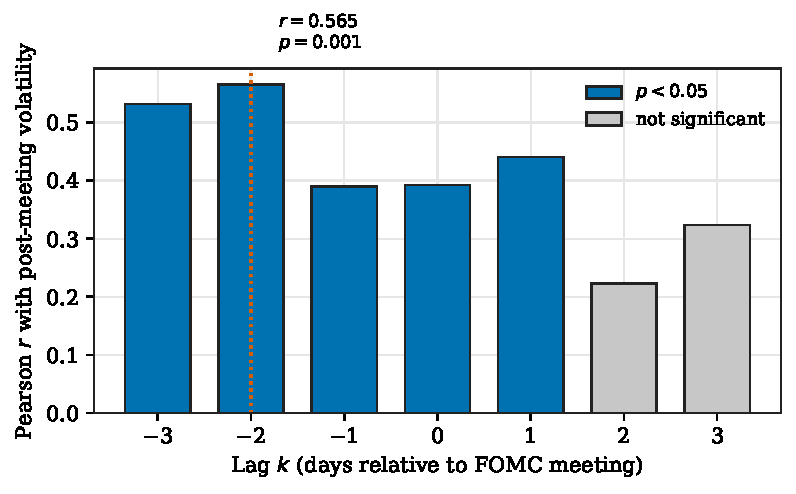
\includegraphics[width=0.62\textwidth]{fig1_leadlag_gdelt.pdf}
\caption{Lead--lag profile, broad corpus. Pearson $r$ between media--FOMC cosine
similarity and post-meeting S\&P 500 realized volatility at each lag $k$
($n=33$ meetings). Filled bars are significant at the five percent level; the
dotted line marks the pre-specified lag $k=-2$.}
\label{fig:leadlag}
\end{figure}

\begin{table}[t]
\centering
\caption{Lead--lag correlations around the meeting, broad corpus.}
\label{tab:leadlag}
\small
\begin{tabular}{rrrrr}
\toprule
Lag $k$ & $N$ & Mean cosine & Pearson $r$ & $p$-value \\
\midrule
-3 & 33 & 0.058 & 0.532*** & 0.0014 \\
-2 & 33 & 0.073 & 0.565*** & 0.0006 \\
-1 & 33 & 0.074 & 0.390** & 0.0249 \\
+0 & 33 & 0.079 & 0.392** & 0.0239 \\
+1 & 33 & 0.079 & 0.441** & 0.0103 \\
+2 & 33 & 0.074 & 0.223 & 0.2125 \\
+3 & 33 & 0.058 & 0.324* & 0.0659 \\
\bottomrule
\end{tabular}
\vspace{2pt}
\caption*{\footnotesize Stars denote $p<0.10$ ($*$), $p<0.05$ ($**$),
$p<0.01$ ($***$). $n=33$ meetings (2015--2019).}
\end{table}

\subsection{The main regression and the collapse under controls}

Table~\ref{tab:main} is the center of the paper. Column (1) reports the bivariate
relationship, in which a one-unit increase in \simk{-2} is associated with a $4.77$
increase in post-meeting realized volatility; the estimate is significant at one
percent under both HC1 and HAC standard errors, and the regressor alone explains
about a third of the variation. The remaining columns then add controls one at a
time, and the sequence is where the story turns. As soon as we control for
pre-meeting realized volatility in column (2), the coefficient falls to $1.38$ and
loses significance, which tells us that much of the raw association simply reflects
the persistence of volatility across the meeting. Adding the pre-meeting VIX in
column (3) reduces it further to $0.98$ while the $R^2$ rises to $0.64$, so the
prevailing level of implied uncertainty absorbs most of what remains. Neither
pre-meeting tone in column (4) nor the orthogonalized monetary policy surprise in
column (5) revives the coefficient, and the year fixed effects in column (6) leave
it small and insignificant as well. The surprise control is the decisive test:
because the similarity coefficient is already near zero before the surprise enters
and does not move when it does, the pre-meeting signal cannot be read as
information about the announcement that markets had not yet priced. What the raw
correlation captured, in short, is almost entirely the prevailing state of market
uncertainty rather than an independent media channel, and Figure~\ref{fig:coef}
traces the same collapse across all six specifications.

\begin{table}[t]
\centering
\caption{Pre-meeting similarity and post-meeting volatility, broad corpus.}
\label{tab:main}
\small
\begin{tabular}{lcccccc}
\toprule
 & (1) & (2) & (3) & (4) & (5) & (6) \\
\midrule
$\mathrm{sim}_{-2}$ & 4.768*** & 1.379 & 0.977 & 1.050 & 0.690 & 0.728 \\
\quad HC1 SE & (1.171) & (1.391) & (1.335) & (1.547) & (1.553) & (1.885) \\
\quad HAC SE & (1.249) & (1.143) & (1.084) & (1.258) & (1.140) & (1.571) \\
\midrule
Pre-meeting volatility &  & \checkmark & \checkmark & \checkmark & \checkmark & \checkmark \\
Pre-meeting VIX &  &  & \checkmark & \checkmark & \checkmark & \checkmark \\
Pre-meeting sentiment &  &  &  & \checkmark & \checkmark & \checkmark \\
Policy surprise (orth.) &  &  &  &  & \checkmark & \checkmark \\
Year fixed effects &  &  &  &  &  & \checkmark \\
\midrule
$R^2$ & 0.319 & 0.546 & 0.639 & 0.639 & 0.657 & 0.695 \\
$N$ & 33 & 33 & 33 & 33 & 33 & 33 \\
\bottomrule
\end{tabular}
\vspace{2pt}
\caption*{\footnotesize Dependent variable: post-meeting realized volatility.
Column (5) adds the orthogonalized Bauer--Swanson monetary policy surprise. HC1 and
Newey--West (HAC, two lags) standard errors in parentheses. Stars denote
$p<0.10$ ($*$), $p<0.05$ ($**$), $p<0.01$ ($***$). $n=33$.}
\end{table}

\begin{figure}[t]
\centering
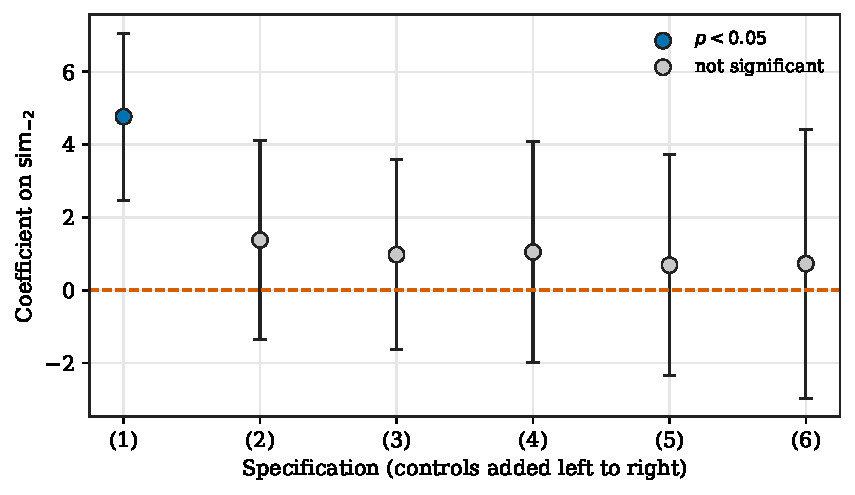
\includegraphics[width=0.62\textwidth]{fig3_coefficient_path.pdf}
\caption{Coefficient on \simk{-2} across specifications (1) to (5) of
Table~\ref{tab:main}, with ninety-five percent HC1 intervals. The point estimate
falls by roughly four-fifths once pre-meeting volatility and the VIX are included.}
\label{fig:coef}
\end{figure}

\subsection{Identification}

Table~\ref{tab:id} collects the identification tests, and Figure~\ref{fig:placebo}
shows the permutation null. The raw correlation of $0.56$ sits far in the right
tail of the permutation distribution, with a two-sided permutation $p$-value of
$0.0006$, so the unconditional signal is not an artifact of chance re-pairing. The
partial correlation given pre-meeting volatility and the VIX, however, is $0.14$
with a permutation $p$-value of $0.42$, indistinguishable from the null. The
bootstrap tells the same story: the ninety-five percent interval for the bivariate
coefficient is $[2.33,\,6.90]$ and excludes zero, while the interval for the
controlled coefficient is $[-1.99,\,3.24]$ and does not. The Granger tests give
only marginal evidence of temporal precedence, significant at the second lag
($p=0.045$) and not at the first, and the leave-one-out slope for the bivariate
relationship stays in a narrow band from $4.12$ to $5.32$, so the result is not
driven by any single meeting. Taken together, the battery says that the pre-meeting
association is genuine but is not separable from the common macro-uncertainty
state.

\begin{figure}[t]
\centering
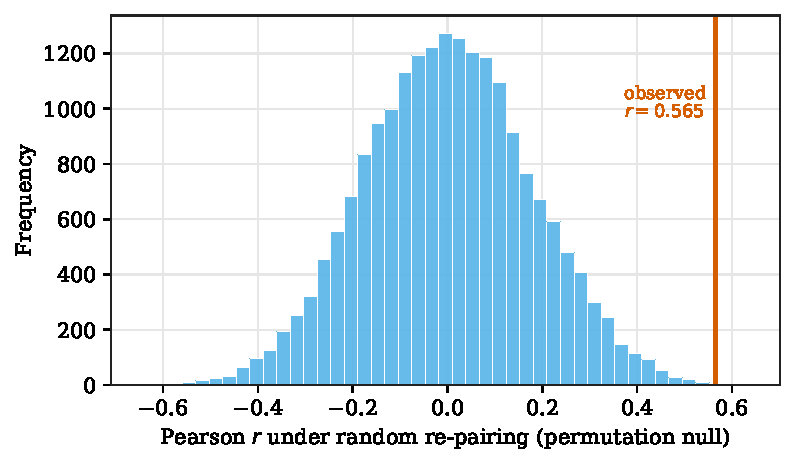
\includegraphics[width=0.62\textwidth]{fig4_placebo_null.pdf}
\caption{Permutation placebo. Distribution of the correlation between \simk{-2} and
post-meeting volatility under twenty thousand random re-pairings; the vertical line
is the observed value.}
\label{fig:placebo}
\end{figure}

\begin{table}[t]
\centering
\caption{Identification battery, broad corpus.}
\label{tab:id}
\small
\begin{tabular}{llr}
\toprule
Check & Statistic & Value \\
\midrule
Permutation placebo & raw corr., perm. $p$ & 0.565 ($p=0.0006$) \\
 & partial corr. $\mid$ VIX, vol., perm. $p$ & 0.145 ($p=0.422$) \\
Granger $\text{sim}\to\text{vol}$ & lag 1, $F$-test $p$ & 1.24 ($p=0.274$) \\
Granger $\text{sim}\to\text{vol}$ & lag 2, $F$-test $p$ & 3.51 ($p=0.045$) \\
Granger $\text{sim}\to\text{vol}$ & lag 3, $F$-test $p$ & 2.43 ($p=0.092$) \\
Bootstrap (bivariate) & 95\% CI for $\beta$ & [2.33, 6.90] \\
Bootstrap (controlled) & 95\% CI for $\beta$ & [-1.99, 3.24] \\
\bottomrule
\end{tabular}
\end{table}

\subsection{Source heterogeneity}

Figure~\ref{fig:sources} overlays the lead--lag profiles of the three corpora.
The broad corpus produces the significant pre-meeting pattern; the two curated
outlets do not, at any pre-meeting lag. This holds even though the curated outlets
show higher same-day topical similarity, which is what we expect if their editorial
focus keeps individual articles close to Fed language while their small volume
leaves too few meetings at any given lag to detect a lead--lag relationship. The
population-scale signal is a property of breadth and volume, not of curation.

\begin{figure}[t]
\centering
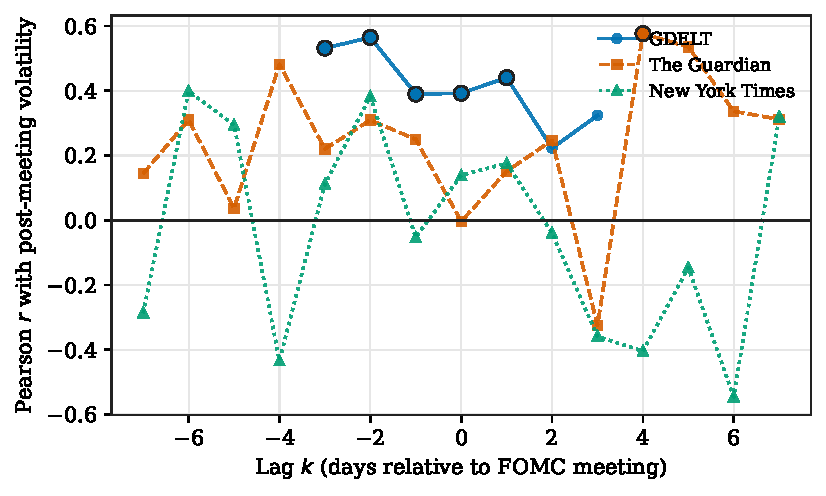
\includegraphics[width=0.62\textwidth]{fig2_leadlag_sources.pdf}
\caption{Lead--lag profiles by source. Pearson $r$ against post-meeting volatility
at each lag for the broad corpus, The Guardian, and The New York Times. Filled
markers are significant at the five percent level.}
\label{fig:sources}
\end{figure}

\subsection{Regime and subsample robustness}

Table~\ref{tab:sub} reports subsamples. The unconditional relationship is strongest
in the Yellen-era meetings ($\hat\beta=5.54$, $n=24$, $p<0.001$) and is weak and
imprecise in the small Powell-era window ($n=9$). Splitting by the pre-meeting VIX,
the relationship is significant in the low-VIX half ($\hat\beta=2.78$, $p=0.006$)
and not in the high-VIX half, which is consistent with the controlled result: when
uncertainty is already high, the similarity measure adds little beyond the level of
the VIX itself. The leave-one-out range confirms the bivariate slope is stable
across the sample.

\subsection{Alternative volatility windows}

Because the choice of a post-meeting window is a modeling decision, we re-estimate
the relationship with the outcome measured over three, five, seven, and ten trading
days. Table~\ref{tab:altwin} and Figure~\ref{fig:altwin} report the pattern, and it
is the same at every window. The bivariate slope is positive throughout, reaching
significance at the five-day window and remaining marginal at seven and ten days,
whereas the controlled slope, which conditions on pre-meeting volatility and the
VIX, is indistinguishable from zero at every window and even changes sign at the
shortest. The headline result is therefore not an artifact of a particular
volatility horizon: the unconditional signal survives the choice of window, and the
conditional signal disappears regardless of it.

\begin{table}[t]
\centering
\caption{Robustness to the post-meeting volatility window.}
\label{tab:altwin}
\small
\begin{tabular}{rrcccc}
\toprule
 & & \multicolumn{2}{c}{Bivariate} & \multicolumn{2}{c}{Controlled} \\
\cmidrule(lr){3-4}\cmidrule(lr){5-6}
Window (days) & $N$ & $\hat\beta$ & $p$ & $\hat\beta$ & $p$ \\
\midrule
3 & 33 & 2.431 & 0.205 & -1.109 & 0.731 \\
5 & 33 & 5.108** & 0.027 & 0.454 & 0.865 \\
7 & 33 & 3.764* & 0.092 & -0.874 & 0.656 \\
10 & 33 & 3.734* & 0.064 & 0.082 & 0.959 \\
\bottomrule
\end{tabular}
\vspace{2pt}
\caption*{\footnotesize HC1 standard errors. Stars denote $p<0.10$ ($*$),
$p<0.05$ ($**$), $p<0.01$ ($***$). Controlled columns condition on pre-meeting
volatility and the pre-meeting VIX. $n=33$.}
\end{table}

\begin{figure}[t]
\centering
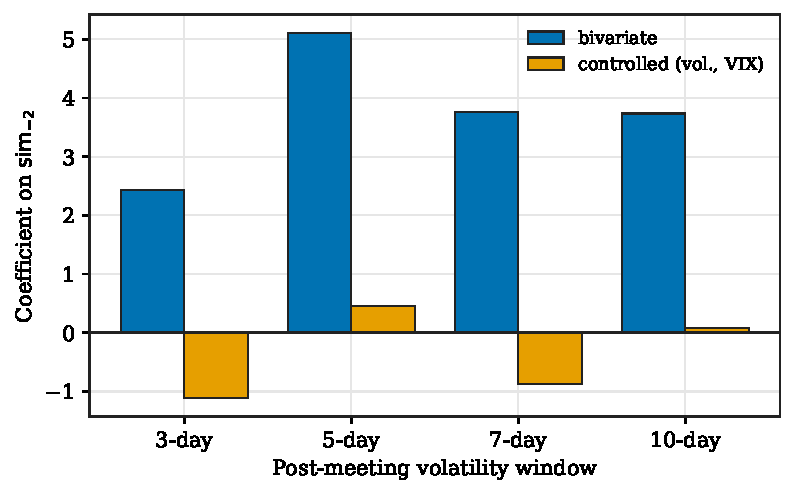
\includegraphics[width=0.6\textwidth]{fig9_altwindow.pdf}
\caption{Coefficient on \simk{-2} across post-meeting volatility windows. The
bivariate estimate is positive at every window; the controlled estimate is near
zero throughout.}
\label{fig:altwin}
\end{figure}

\begin{table}[t]
\centering
\caption{Subsample estimates of the \simk{-2} coefficient.}
\label{tab:sub}
\small
\begin{tabular}{lrrr}
\toprule
Subsample & $N$ & $\hat\beta_{\mathrm{sim}_{-2}}$ & $p$ \\
\midrule
full (bivariate) & 33 & 4.768*** & 0.000 \\
full (controlled) & 33 & 0.977 & 0.464 \\
Yellen (bivariate) & 24 & 5.536*** & 0.000 \\
Powell (bivariate) & 9 & 1.221 & 0.764 \\
high VIX (bivariate) & 17 & 2.792 & 0.152 \\
low VIX (bivariate) & 16 & 2.779*** & 0.006 \\
leave-one-out range (bivariate) & 33 & min=4.117, max=5.322 & \\
\bottomrule
\end{tabular}
\vspace{2pt}
\caption*{\footnotesize HC1 standard errors. Stars denote $p<0.10$ ($*$),
$p<0.05$ ($**$), $p<0.01$ ($***$).}
\end{table}

\subsection{Market validation of the tone measure}

Because the tone of the minutes is measured with an externally fixed market
dictionary, the right test of the measure is not whether it agrees with a second
word list but whether it moves with the market, and it does. Across all 88 meetings
the negative intensity of the minutes, counted with the Loughran--McDonald negative
category, rises with the level of implied volatility on the eve of the meeting
($r=0.52$, $p<10^{-6}$); it is followed by higher realized volatility in the week
after the meeting ($r=0.39$, $p<0.001$); and the net of positive over negative
intensity carries the same information with the opposite sign, correlating at
$-0.37$ with post-meeting volatility ($p<0.001$). The measure also lines up with the
market's own reading of the decision itself. Over the 72 meetings for which the
high-frequency surprise is available, minutes written in more negative language
precede larger-magnitude policy surprises ($r=0.37$, $p=0.001$), whereas the signed
net tone is unrelated to the signed surprise ($r=0.07$, $p=0.53$); the contrast is
exactly what one expects if the operative channel is the scale of uncertainty in
the language rather than its direction. Figure~\ref{fig:tone} plots the tightest of
these relationships, between negative tone and the pre-meeting VIX, and the tone
timeline in the appendix recovers the known turning points with no hand-labeling,
the most negative readings falling on the March and April 2020 emergency meetings
and the language turning steadily more negative through the 2022--2023 tightening.
That a market dictionary applied to the Committee's own words should track the
market's gauges of uncertainty is the measurement counterpart of the paper's
central reading: the negative, uncertainty-laden language that fills the minutes in
turbulent periods is written at the same time, and for the same reason, that the
market's implied volatility is elevated.

The result does not depend on the dictionary. Scoring the same minutes with the
fine-tuned FinBERT-tone transformer, which reads each passage in context rather than
counting words, reproduces both facts: the model's negative-tone probability rises
with the pre-meeting VIX ($r=0.47$, $p<10^{-5}$) and forecasts post-meeting realized
volatility ($r=0.34$, $p=0.001$), and it agrees closely with the dictionary measure,
correlating at $0.76$ with negative intensity and $0.74$ with net tone across the 88
meetings. The contextual model attaches somewhat less weight to the policy surprise
than the dictionary does, and its association with the surprise magnitude is
positive but insignificant, but the two measurement strategies agree on the one
relationship that carries the interpretation, the tie between the Committee's
negative language and the market's uncertainty state.

\begin{figure}[t]
\centering
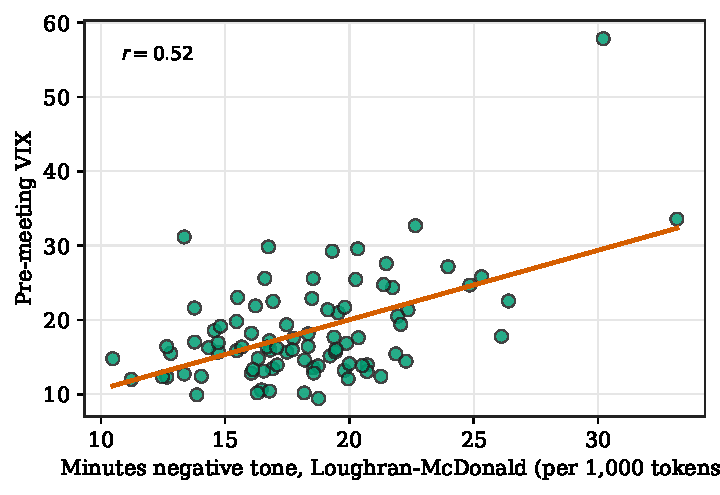
\includegraphics[width=0.52\textwidth]{fig7_sentiment_agreement.pdf}
\caption{Market validation of tone. Negative intensity of the FOMC minutes, counted
with the Loughran--McDonald negative category per thousand tokens, against the
pre-meeting VIX across the 88 meetings; the positive slope ties the Committee's own
language to the market's forward-looking uncertainty gauge.}
\label{fig:tone}
\end{figure}

\begin{table}[t]
\centering
\caption{Sentiment scorer throughput on a five-million-token workload.}
\label{tab:bench}
\small
\begin{tabular}{lrr}
\toprule
Implementation & Time (s) & Speedup \\
\midrule
Pure Python loop & 0.241 & 1.0$\times$ \\
NumPy searchsorted & 0.123 & 2.0$\times$ \\
Numba parallel JIT & 0.009 & 26.8$\times$ \\
\bottomrule
\end{tabular}
\end{table}

% =====================================================================
\section{Discussion}
\label{sec:discussion}

The results support a specific and disciplined reading of anticipation. There is a
genuine pre-meeting signal in the national news stream: two days before a meeting,
media coverage that more closely resembles the eventual FOMC minute is followed by
higher realized volatility, the pattern is located before the announcement, and it
is robust to permutation, bootstrap, and leave-one-out inference. But the signal is
not an independent media channel. It is absorbed almost entirely by the prevailing
level of implied volatility and by recent realized volatility, and the partial
association given those controls is indistinguishable from noise. The most
defensible mechanism is joint determination through a common latent state. When
macroeconomic uncertainty is elevated on the eve of a meeting, the news stream
naturally produces more Fed-adjacent, Fed-resembling language, and markets
simultaneously price a wider distribution of outcomes; both are reading the same
environment. This is the rational-inattention logic of
\citet{sims2003implications} and \citet{mackowiak2009optimal} applied to a discrete
policy event: attention, of journalists and investors alike, flows toward the
high-variance signal, and the FOMC meeting is the moment that signal is at its
sharpest. The tone evidence is the measurement counterpart of this reading and is
worth dwelling on, because it is independent of the similarity result and rests on
a market dictionary rather than a bespoke list. When the minutes are scored with
the Loughran--McDonald negative category, their negativity co-moves strongly with
the pre-meeting VIX, at a correlation of roughly one-half, and forecasts the
realized volatility that follows, and it tracks the magnitude, though not the sign,
of the high-frequency policy surprise. The Committee's own language, in other words, is most negative and
most uncertainty-laden precisely in the states where the market's priced
uncertainty is highest, which is difficult to reconcile with a story in which the
text carries information the market does not already hold and easy to reconcile
with the common-state reading, in which the minutes and the market are two
readings of the same macroeconomic environment.

This reading differs from a causal media-to-market story and it should. We have no
instrument that shifts coverage without shifting the Fed or the economy, and the
Granger evidence is only marginal, so we do not claim that journalism moves prices.
The reading also refines the source-heterogeneity result. The broad corpus leads
and the curated outlets do not, not because broad coverage is better but because it
is larger: with more meetings covered at each lag, the common-state signal is
estimable, whereas a few dozen articles from one outlet leave too little power to
see it. That is a statement about measurement at scale, and it is the practical
payoff of building the population corpus rather than a sample of it. For the Fed,
the implication is modest but real. A meeting communications calendar operates in
an environment where the market's uncertainty is already visible in the VIX before
the Committee speaks; the value of communication is in resolving that uncertainty,
and indeed volatility falls after most meetings in our sample, with the emergency
cut of March 2020 and the first large hike of 2022 the notable exceptions.

% =====================================================================
\section{Conclusion}
\label{sec:conclusion}

At the scale of United States Federal Reserve news coverage, media discourse
around FOMC meetings anticipates the market outcome in a precise sense: pre-meeting
media--FOMC textual similarity is strongly associated with post-meeting volatility,
and the association is located two days before the meeting. The anticipation is not
media causing markets. Once we condition on the prevailing level of uncertainty,
the signal is common macro variation that both the news stream and the market are
processing at once. The finding is invisible at single-outlet scale, where too few
observations exist at any lag to separate the pattern from noise, and it is
defensible only because the identification is staged so the reader can see the
signal weaken as the controls enter.

The study has clear limits. The broad-corpus estimation sample, where pre-meeting
coverage is complete at a common lag, is 33 meetings from 2015 to 2019, and we
report every result on that transparent sample rather than pooling incomplete
windows. The similarity baseline is term-frequency based, and while the contextual-embedding
similarity remains a GPU-bound extension, the contextual tone measure is no longer
only prospective: the FinBERT results above confirm that the market-validated tone
finding survives the move from a dictionary to a transformer. And the design
is descriptive of lead--lag structure rather than causal, by construction. Future
work should therefore extend the complete-coverage window forward and add the
embedding-based similarity and tone measures that the pipeline already permits,
since both are matters of running an existing stage rather than rebuilding the
analysis. The high-frequency policy surprise, which the plan had reserved for later,
is already included here as a control, and the fact that the pre-meeting signal is
absent once common uncertainty is accounted for, with or without that surprise, is
the result we are most confident will carry forward.

% =====================================================================
\section*{Declarations}

\noindent\textbf{CRediT author statement.} Duo Wang: conceptualization, methodology
(econometrics and NLP), formal analysis, validation, investigation, data curation,
writing (original draft and review), project administration. Yuzhao Jin: software,
visualization, methodology (computational architecture), writing (review and
editing, methods architecture).\\
\noindent\textbf{Conflict of interest.} None.\\
\noindent\textbf{Data and code availability.} All code and the committed
intermediate artifacts that reproduce every table and figure are in the project
repository; the CPU pipeline regenerates the results with a single Snakemake
command. Raw GDELT records are available from the AWS Open Data registry, the
curated-outlet coverage through the respective article APIs, the CBOE Volatility
Index and daily S\&P 500 series from public market-data sources, and the
high-frequency monetary policy surprises from the Federal Reserve Bank of San
Francisco \citep{bauer2023reassessment}. The FOMC minutes are retrieved from the
Federal Reserve's public archive and cached with the package, and the tone measure
uses the publicly distributed Loughran--McDonald master dictionary
\citep{loughran2011liability}.

% =====================================================================
\bibliographystyle{apalike}
\bibliography{references}

\end{document}
